\section{自己紹介}
こんにちは,ゆひ(@HSAU\_ Dosei)です. 普段はUnityでARアプリ作ってます. 今年も同人誌を書く話になったのでUnityのマスクシェーダーを書いて遊んでみました. 軽めなのでおまけ程度だと思って読んでください.
\section{どんなShader?}
消したいObjectに適用することでそのObjectが消えるShaderです.

白黒で分かりづらいかもしれませんが,こんな感じで重なっている部分が消えて後ろが透けて見えています.
\begin{figure}[htbp]
\centering
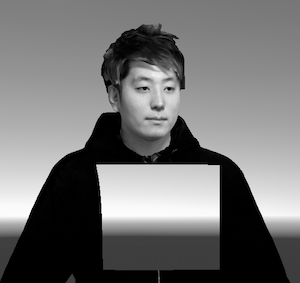
\includegraphics[width=5cm,height=5cm]{./assets/yuhiasset/hsau_dosei2.png}
\end{figure}

\newpage

\section{まずShaderを書こう}
\begin{figure}[h]
\centering

\includegraphics[]{./assets/yuhiasset/hsau_dosei1.png}
\caption{Shader}
\label{fig:shader}
\end{figure}
Assets/Create/Shader/Standard Surface ShaderからShaderを作成し名前をつけます.
今回はStelthとします.
一旦中身を消してから中身を記述してあげます!!!
そして作成したShader(図:\ref{fig:shader})を選択し,Create/Material からMaterialを作成します.
Materialの名前は,好きにつけてもらって大丈夫です.
あとはこのMaterialをマスクしたいObjectにつけてあげれば消えます!!

\begin{minted}[frame=lines,framesep=2mm,baselinestretch=1.2,fontsize=\footnotesize,linenos,breaklines]{text}
Shader "Custom/Stealth" {
            SubShader {
                Tags { "RenderType"="Opaque" "Queue"="Geometry-1"}
                Pass{

            ColorMask 0

            CGPROGRAM
            #pragma vertex vert
            #pragma fragment frag
            struct appdata{
                float4 vertex : POSITION;
            };
            struct v2f{
                float4 pos : SV_POSITION;
            };
            v2f vert(appdata v){
                v2f o;
                o.pos = UnityObjectToClipPos(v.vertex);
                return o;
            }
            half4 frag (v2f i) : COLOR{
                return half4(0,0,0,0);
            }
            ENDCG
        }
        
    }
}
\end{minted}

\section{書けたらさっそく使うぞ!!}
さて先程書いてもらったこのShaderですが$\cdots \cdots$
{\bf 何に使えるの?????}
実際このShaderは普通にUnityやっていればあまり使いみちが無いと思います.
しかし、このShaderはARになった途端\bf{化けます}.

\subsection{ex どこでもドア}
\begin{figure}[htbp]
\centering
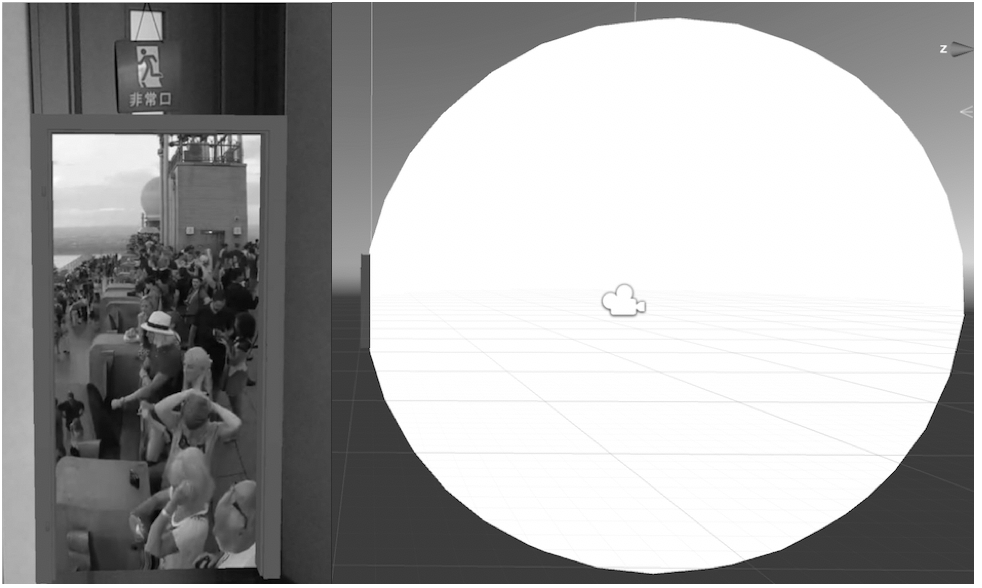
\includegraphics[width=3cm,height=3cm]{./assets/yuhiasset/hsau_dosei3.png}
\end{figure}
この場合、現実世界ではドアのフレームしか見えていませんが,実際には後ろにSphereがあります.
当たり前ですが,普通にドアのフレームとSphereを置いただけではドアの後ろにあるSphereが見えてしまいます.そこで先程のShaderをつけたObjrctをドアの周りに配置してマスクすることでドアだけが見えるようになります.
このようにARの場合,ある一定方向から見えてはいけないけど置かないといけないObjectを置かなければならない状況になる場合があります.そういった時にこのShaderはとても{\bf 輝く}のです.

\subsection{ex 空間をマスク}
\begin{figure}[h]
\centering
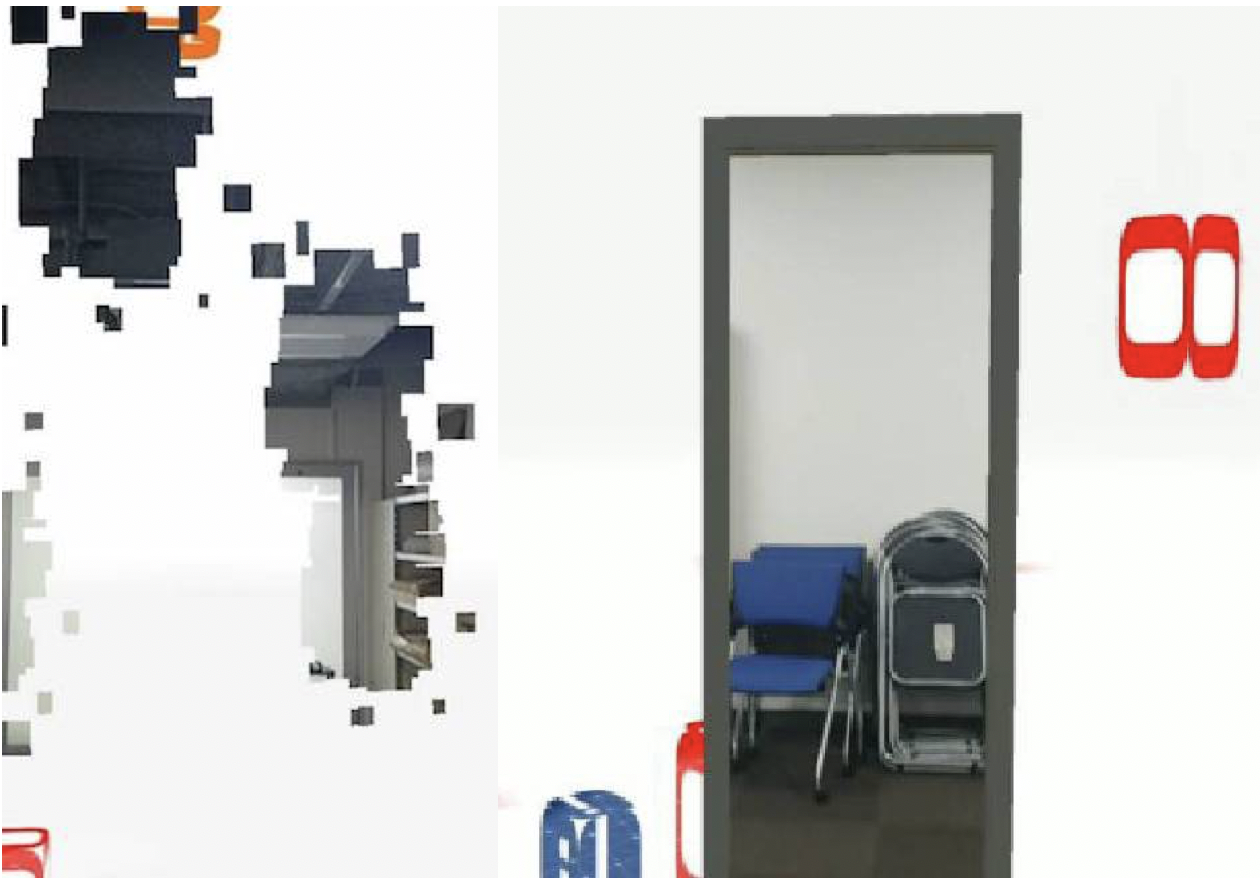
\includegraphics[width=5cm,height=5cm]{./assets/yuhiasset/hsau_dosei6.png}
\end{figure}
この例では外から空間を見るどこでもドアとは対象的にこの例では空間から外を見ています.
通常のARアプリは向こうの世界を覗く,キャラクターがやってくる,といったものが多いと思います.
しかし,その逆をやっているものはほとんどありません.なぜなら空間全てを覆ってしまうとそれはもはや{\bf AR}と呼べなくなってしまうから.{\bf AR}の良い所は現実の空間を{\bf 拡張}することで普段ありえないような体験ができることだと僕は考えます,程よく現実世界を露出させてあげるとすごく{\bf エモく}
なります.
そこでこのShaderでマスクすることで現実世界が露出し{\bf エモさ}が増すのです.

\section{最後に}
結局Shaderの話ではなくARの話になってしまいましたが,きっとマスクシェーダーを用いることでできるようになる表現について分かってもらえたと\sout{勝手}に思っています。
今回はARでの使用例について取り上げましたが,他にもまだまだ使いみちがあるはずです!

{\bf 組み合わせは無限大!君の想像次第で無限に使えるぞ!}

ゆひ
